\documentclass[tikz,border=15pt]{standalone}
\usepackage{helvet}
\renewcommand{\familydefault}{\sfdefault}
\usepackage{tikz}
\usetikzlibrary{positioning, fit, calc, shapes.geometric, decorations.pathreplacing, arrows.meta, backgrounds, matrix}

\definecolor{emeraldpine}{HTML}{1A4D3E}
\definecolor{harvardcrimson}{HTML}{A51C30}
\definecolor{ethdarkblue}{HTML}{1F407A}
\definecolor{ethpetrol}{HTML}{007A87}
\definecolor{ethbronze}{HTML}{B87333}
\definecolor{ethpurple}{HTML}{5B4B8A}
\definecolor{ink}{HTML}{1A202C}
\definecolor{softink}{HTML}{4A5568}
\definecolor{paleink}{HTML}{A0AEC0}
\definecolor{cardbg}{HTML}{F8FAFC}
\definecolor{shadecolor}{HTML}{F4F6F9}

% ASIL colors
\definecolor{asild}{HTML}{A51C30} % harvardcrimson
\definecolor{asilc}{HTML}{D35400} % Dark Orange
\definecolor{asilb}{HTML}{F39C12} % Orange-Yellow
\definecolor{asila}{HTML}{27AE60} % Green
\definecolor{asilqm}{HTML}{7F8C8D} % Gray

\begin{document}
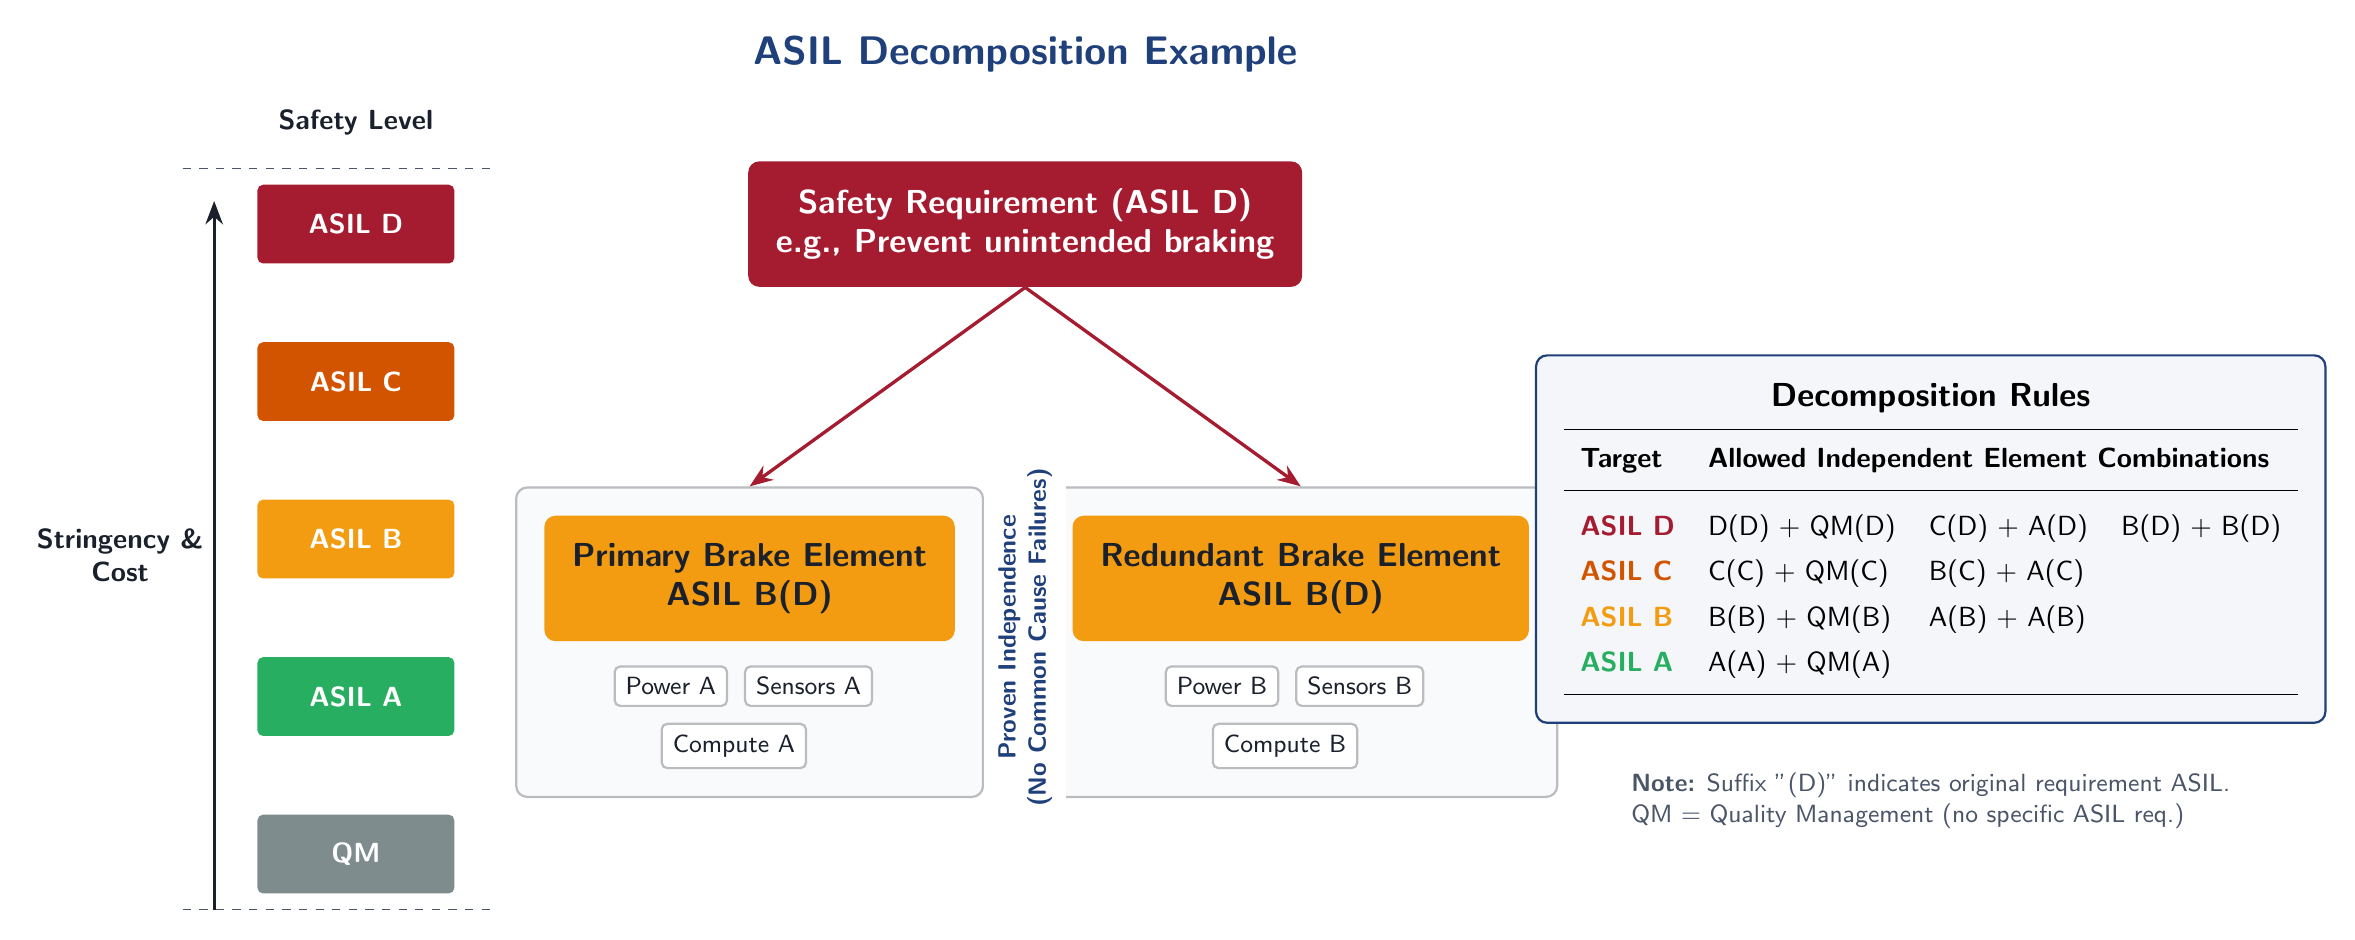
\begin{tikzpicture}[
    font=\sffamily,
    >=Stealth,
    box/.style={draw=ink!30, thick, rounded corners, align=center, fill=cardbg, text=ink, inner sep=8pt},
    reqbox/.style={draw=none, rounded corners, align=center, text=white, inner sep=10pt, font=\bfseries\large},
    smallbox/.style={draw=ink!30, thick, rounded corners=2pt, align=center, fill=white, text=ink, inner sep=4pt, font=\small},
    scalebox/.style={draw=none, rounded corners=2pt, text=white, font=\bfseries, align=center, minimum width=2.5cm, minimum height=1cm},
    tablebox/.style={draw=ethdarkblue, thick, rounded corners, fill=shadecolor, inner sep=10pt},
]

% 1. Vertical Scale (Left)
\node[scalebox, fill=asild] (sd) at (0, 8) {ASIL D};
\node[scalebox, fill=asilc] (sc) at (0, 6) {ASIL C};
\node[scalebox, fill=asilb] (sb) at (0, 4) {ASIL B};
\node[scalebox, fill=asila] (sa) at (0, 2) {ASIL A};
\node[scalebox, fill=asilqm] (sqm) at (0, 0) {QM};

\draw[->, very thick, ink] (sqm.south) ++(-1.8,-0.2) -- ++(0, 9) node[midway, left, align=center, font=\bfseries] {Stringency \&\\Cost};
\draw[dashed, softink] (sqm.south) ++(-2.2, -0.2) -- ++(4, 0);
\draw[dashed, softink] (sd.north) ++(-2.2, 0.2) -- ++(4, 0);

\node[font=\bfseries, text=ink, above=0.5cm of sd] {Safety Level};

% 2. Decomposition Example (Center)
\node[reqbox, fill=asild, minimum width=6cm] (req) at (8.5, 8) {Safety Requirement (ASIL D)\\e.g., Prevent unintended braking};

% Left Element
\node[reqbox, fill=asilb, minimum width=4cm, text=ink] (elem1) at (5, 3.5) {Primary Brake Element\\ASIL B(D)};
\node[smallbox, below=0.3cm of elem1, xshift=-1cm] (p1) {Power A};
\node[smallbox, right=0.2cm of p1] (s1) {Sensors A};
\node[smallbox, below=0.2cm of p1, xshift=0.8cm] (c1) {Compute A};
\node[fit=(elem1)(p1)(s1)(c1), box, inner sep=10pt] (sys1) {};
% redraw elem1 over fit
\node[reqbox, fill=asilb, minimum width=4cm, text=ink] at (5, 3.5) {Primary Brake Element\\ASIL B(D)};
\node[smallbox] at (p1) {Power A};
\node[smallbox] at (s1) {Sensors A};
\node[smallbox] at (c1) {Compute A};

% Right Element
\node[reqbox, fill=asilb, minimum width=4cm, text=ink] (elem2) at (12, 3.5) {Redundant Brake Element\\ASIL B(D)};
\node[smallbox, below=0.3cm of elem2, xshift=-1cm] (p2) {Power B};
\node[smallbox, right=0.2cm of p2] (s2) {Sensors B};
\node[smallbox, below=0.2cm of p2, xshift=0.8cm] (c2) {Compute B};
\node[fit=(elem2)(p2)(s2)(c2), box, inner sep=10pt] (sys2) {};
% redraw elem2 over fit
\node[reqbox, fill=asilb, minimum width=4cm, text=ink] at (12, 3.5) {Redundant Brake Element\\ASIL B(D)};
\node[smallbox] at (p2) {Power B};
\node[smallbox] at (s2) {Sensors B};
\node[smallbox] at (c2) {Compute B};

% Decomposition arrows
\draw[->, very thick, asild] (req.south) -- (sys1.north);
\draw[->, very thick, asild] (req.south) -- (sys2.north);

% Independence Barrier
\draw[ultra thick, ethdarkblue, dashed] (8.5, 5) -- (8.5, 0.5) node[midway, fill=white, inner sep=5pt, text=ethdarkblue, font=\bfseries\small, align=center, rotate=90] {Proven Independence\\(No Common Cause Failures)};

\node[font=\bfseries\Large, text=ethdarkblue, above=1cm of req] {ASIL Decomposition Example};

% 3. Rules Table (Right)
\node[tablebox] (table) at (20, 4) {
    \begin{tabular}{l l l l}
        \multicolumn{4}{c}{\textbf{\large Decomposition Rules}} \\[1ex]
        \hline\\[-1.5ex]
        \textbf{Target} & \multicolumn{3}{l}{\textbf{Allowed Independent Element Combinations}} \\[1ex]
        \hline\\[-1ex]
        \textcolor{asild}{\textbf{ASIL D}} & D(D) + QM(D) & C(D) + A(D) & B(D) + B(D) \\[1ex]
        \textcolor{asilc}{\textbf{ASIL C}} & C(C) + QM(C) & B(C) + A(C) & \\[1ex]
        \textcolor{asilb}{\textbf{ASIL B}} & B(B) + QM(B) & A(B) + A(B) & \\[1ex]
        \textcolor{asila}{\textbf{ASIL A}} & A(A) + QM(A) & & \\[1ex]
        \hline
    \end{tabular}
};

\node[font=\small, text=softink, align=left, below=0.5cm of table] {
    \textbf{Note:} Suffix "(D)" indicates original requirement ASIL.\\
    QM = Quality Management (no specific ASIL req.)
};

\end{tikzpicture}
\end{document}
